
\chapter{Gráficas sencillas con Maple 15}
%Entorno para indicar la unidad bibliografica que va a utilizar[estilo de bibliografía]
\begin{bibunit}[plain]

\emph{Maple} es considerado un \emph{Sistema de Álgebra Computacional}, proporciona múltiples
funcionalidades al usuario entre las que se pueden listar las siguientes:

Las siguientes instrucciones nos permiten definir una función y generar su gráfica 
em Maple 15:

\begin{verbatim}
k:= x -> sin(x) + exp(cos(exp(x)));

plot(k(x), x=-10..4.5);
\end{verbatim}

Estas instrucciones nos permiten generar la gráfica que se muestra en la figura \ref{cap1f1}.

\begin{figure}[h!]
\centering
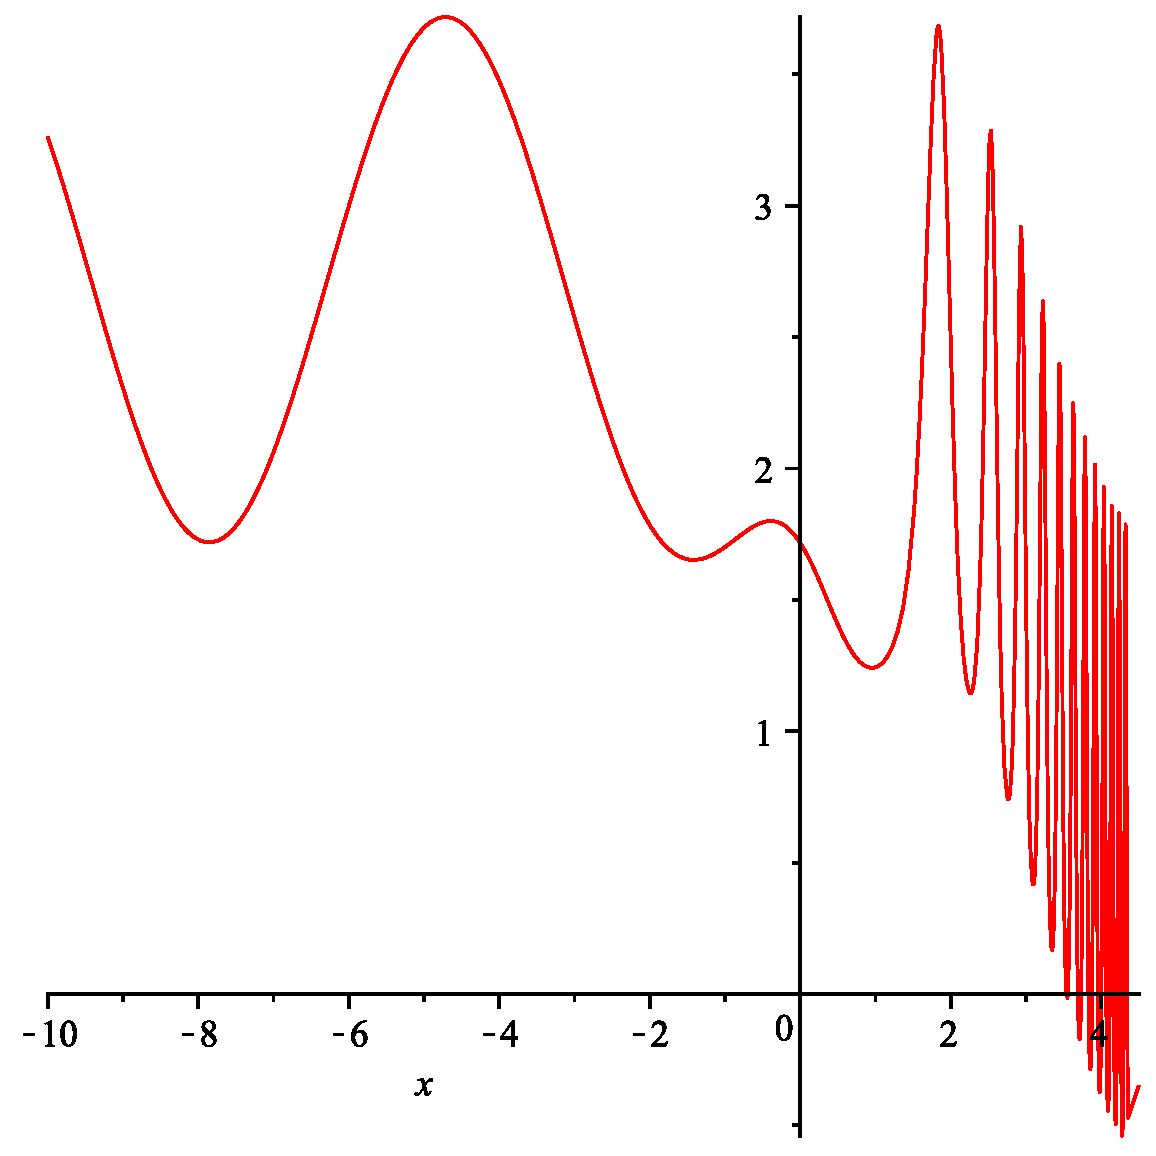
\includegraphics[scale=0.45]{grafica01}
\caption{Gráfica de $sen \left( x \right) +{{\rm e}^{\cos \left( {{\rm e}^{x}} \right) }}$}\label{cap1f1}
\end{figure}

\pagebreak

Veamos otro ejemplo:

Las siguientes instrucciones nos permiten generar la gráfica de la función 
$\displaystyle {x}^{4}\sin \left( {x}^{3} \right) -{x}^{3}\cos \left( {x}^{2}
 \right) +{x}^{2}\sin \left( x \right) -x$

\begin{verbatim}
plot(x^4*sin(x^3)-x^3*cos(x^2)+x^2*sin(x)-x, x = -1.8 .. 1.8);
\end{verbatim}

La gráfica se muestra en la figura \ref{cap1f2}.

\begin{figure}[h!]
\centering
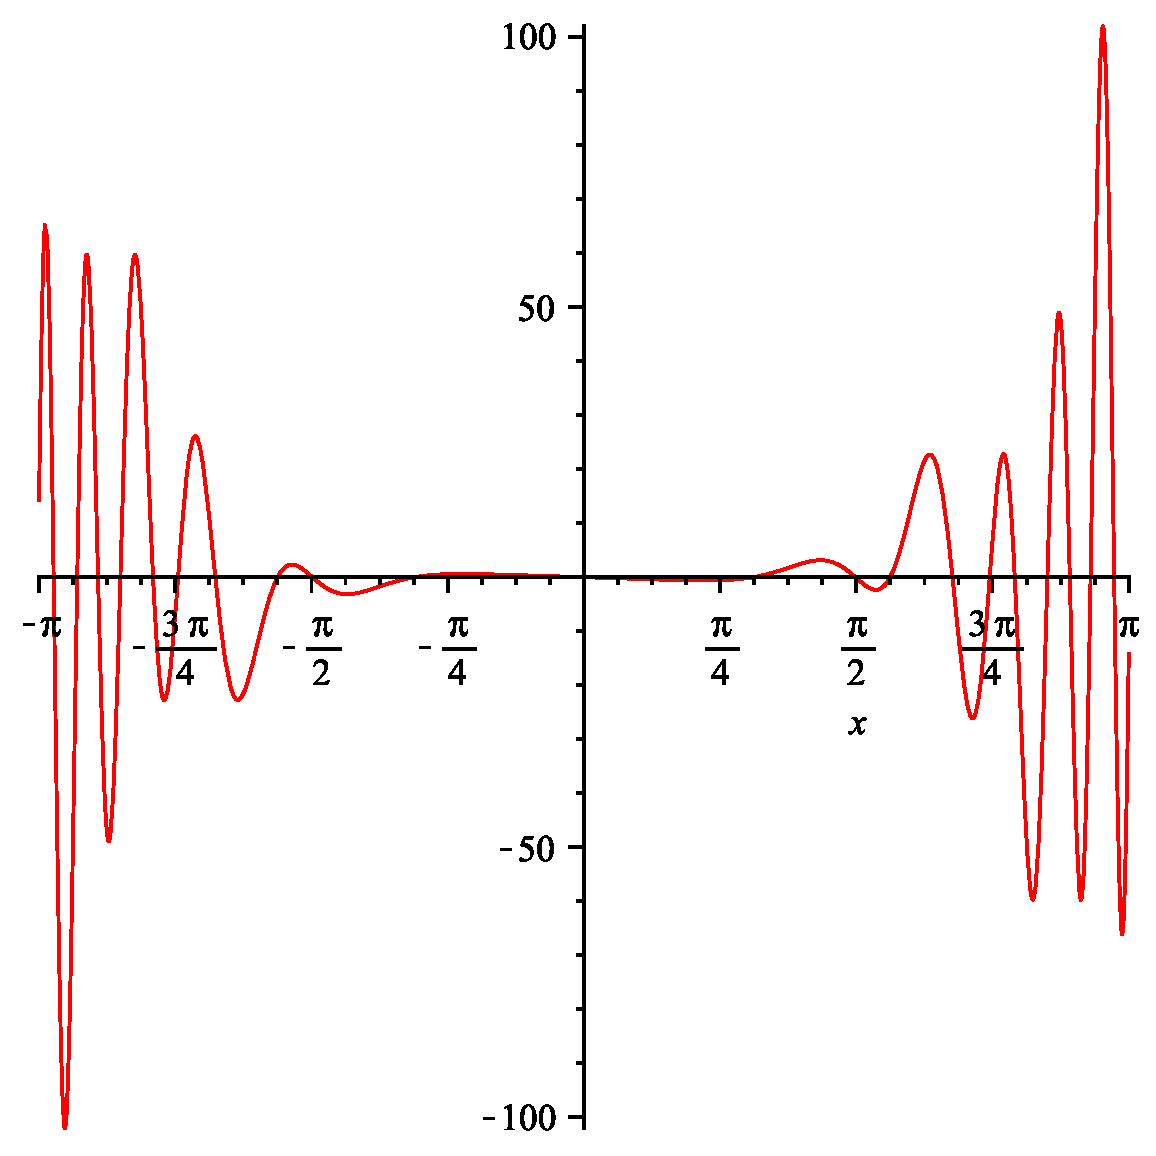
\includegraphics[scale=0.5]{grafica02}
\caption{Gráfica de ${x}^{4}\sin \left( {x}^{3} \right) -{x}^{3}\cos \left( {x}^{2}
 \right) +{x}^{2}\sin \left( x \right) -x$}\label{cap1f2}
\end{figure}

En la tabla \ref{tab:cap1t1} podemos consultar algunas instrucciones de \emph{Maple} que nos
permiten generar gráficas en dos dimensiones. \cite{Lamport}

\begin{table}[h!]
	\caption{Instrucciones de Maple para gráficas en 2D}
	\begin{center}
		\begin{tabular}{|c|c|} \hline
			Instrucción & Tipo de gráfica generada \\ \hline
			plot() & Gráficas en 2D de funciones explicitas \\ \hline
			plot() & Gráficas en 2D de funciones paramétricas \\ \hline
			polarplot() & Gráficas en coordenadas polares \\ \hline
			implicitplot() & Gráficas implícitas en 2D \\ \hline
			complexplot() & Gráficas de expresiones complejas \\ \hline
			contourplot & Gráficas de contornos \\\hline
		\end{tabular}
	\end{center}
	\label{tab:cap1t1}
\end{table}

%Lugar donde va a colocar la bibliografía con putbib[nombreArchivo(s)]
\putbib[mibiblio]
%\addcontentsline{toc}{section}{Bibliografía Cap.1}

\end{bibunit}

